% ##################################################################################################################
\chapter{Tampa, Florida: High Resolution Simulation of Urban Travel and Network Performance for Estimating Mobile Source Emissions}
\label{ch:tampa}
\hfill \textbf{Authors:} Sashikanth Gurram, Abdul R. Pinjari, and Amy L. Stuart

% ##################################################################################################################
\section{Introduction}
Mobile sources are significant contributors to ambient traffic-related air pollution associated with several adverse health impacts in urban areas. Therefore, it is important to accurately characterize mobile source emissions and population exposures to those emissions. Doing so, however, requires a high-resolution simulation of urban travel. In this study, using activity-based travel demand modeling and \gls{matsim}-based dynamic traffic assignment modeling, we demonstrate a large-scale, high-resolution simulation of resident population travel activity and highway network performance in Tampa, Florida. Such high resolution simulation outcomes are useful for subsequent estimation of mobile source emissions and human exposure to those emissions. 

% ##################################################################################################################
\section{Study Area}
Hillsborough County, comprising a majority of the Tampa Bay region in Florida is our study area. The geographic context of the county is presented in Figure~\ref{fig:tampa-fig1}. The freeway road I-275, acts as a major commuter corridor connecting north of Tampa to central business district at the south. The freeway roads I-75 and I-4 run along the north-south and east-west directions, respectively, and serve as major highways for intra-city, inter-city and inter-state travel. The county has a diverse mix of air pollution sources and population demographics, few public transportation options, an unsatisfactory air quality record, and a sprawling urban form, which makes it an interesting test bed from an air pollution perspective.

 %------------
\createfigure%
{The study area of Hillsborough County, Florida}%
{The study area of Hillsborough County, Florida}%
{\label{fig:tampa-fig1}}%
{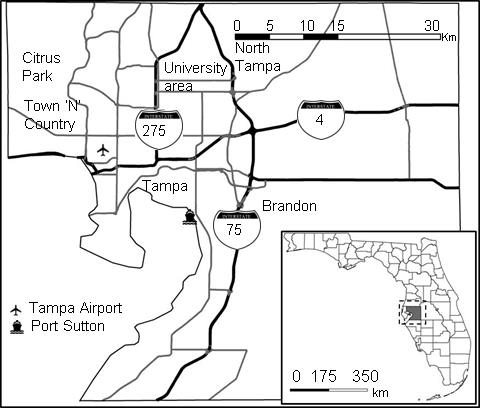
\includegraphics[width=0.7\textwidth, angle=0]{./scenarios/figures/tampa-fig1.jpg}}%
{\citet[][]{GurramEtAl_AQAH_2015}}
 %------------

% ##################################################################################################################
\section{Modeling Framework}
Figure~\ref{fig:tampa-fig2} depicts the modeling framework used to simulate urban population activity and transportation network performance for the study region. 
An \gls{abm} of travel demand (DaySim) is coupled with \gls{matsim}, here applied as a \gls{dta} model. 
The DaySim framework was originally developed for the Sacramento region \citep[][]{BradleyEtAl_JOCM_2010} and calibrated for the Tampa Bay region using local household travel data \citep[][]{GliebeEtAl_TRB_2014}. 
An appealing feature of DaySim is its use of fine, parcel-level resolution for representing space, which leads to high spatial resolution in the simulated activity locations.  
Similar to other \glspl{abm}, inputs to DaySim include detailed population demographics, land-use patterns, and transportation system characteristics in the study region. The demographic inputs come from a population synthesizer called \lstinline|PopGen| \citep[][]{PendyalaEtAl_2011} that generates a synthetic population of individuals and households to match aggregate-level distributions of both household- and person-level characteristics from the U.S. Census. 
To generate demographic variables that were not controlled in PopGen (\eg household car ownership and individual employment characteristics), a suite of econometric models estimated using local data were used. 
Taking all the above as inputs, DaySim simulates the daily activity and travel patterns of all residents in the study region, including the timing, duration and location of activities, and the mode of travel between different activity locations. 
We ran the model on an eight-core Windows machine with a 2.8\,GHz Intel Xeon processor and 24\,\gls{gb} \gls{ram}. 
The run time was approximately 5\,hours for the entire Tampa Bay population of about 3\,million individuals.

 %------------
\createfigure%
{The transportation modeling framework}%
{The transportation modeling framework}%
{\label{fig:tampa-fig2}}%
{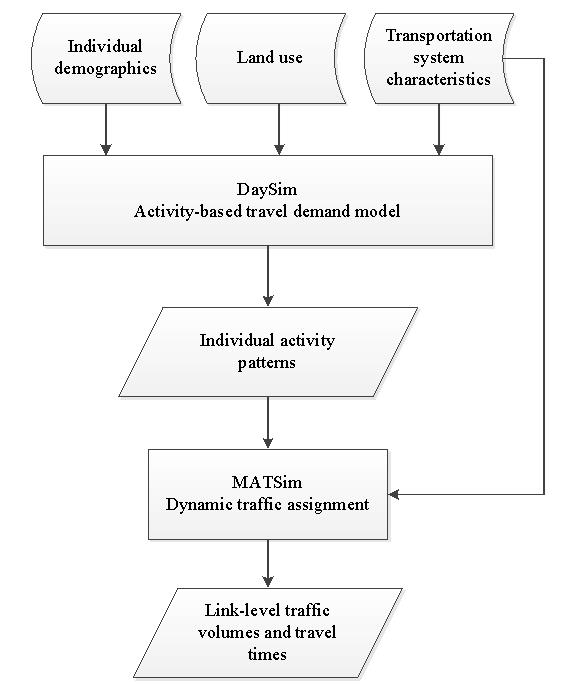
\includegraphics[width=0.7\textwidth, angle=0]{./scenarios/figures/tampa-fig2.jpg}}%
{}
 %------------

DaySim does not simulate the travel route information between the different activity locations. 
However, information on travel routes and network performance (\ie link speeds and volumes) is essential for estimating emissions and human exposure to those emissions. 
Therefore, \gls{matsim} was used to simulate travel routes and network performance \citep[][]{BalmerEtAl_TRBTDF_2008}. 
To do so, outputs from the Tampa \gls{abm} were processed using SPSS and \gls{java} programming to provide the initial set of plans for \gls{matsim}. 
Similarly, the ArcGIS road network file for the Tampa Bay area was processed to create the network inputs for \gls{matsim}. 
Since a majority of travel in Tampa is by automobile (with close to 90\,\% mode share), only the automobile trips were simulated in \gls{matsim}. 
It is worth noting, however, that a rather large number of automobile trips were simulated. 
Specifically, 9.7\,million trips made by approximately 2.3\,million residents of the study region during a 24\,hour period were simulated. 
The simulation was run for 300\,iterations, with the storage capacity factor for the links set to 3. 
Additionally, the maximum plan memory size for each agent was set to 3. The \lstinline|BestScore| and \lstinline|ReRoute| replanning modules were used with a probability of 0.9 and 0.1, respectively. 
To undertake this large-scale and computationally intensive simulation, 48\,parallel processors each with 25\,\gls{gb} of \gls{ram} were utilized from a university research computing cluster setup. 
The total run time for this scenario was approximately 5.2\,days. 
Link-level outputs from the simulation, including the hourly traffic volumes and travel times, were written to a \lstinline|linkstats| file whereas the trip-level route information was written to a \lstinline|plans| file.

% ##################################################################################################################
\section{Results}
The diurnal patterns of link-level passenger car volumes and travel speeds for Hillsborough County are presented in Figure~\ref{fig:tampa-fig3} (in the form of bi-hourly averages). As expected, traffic volumes, shown in Figure~\ref{fig:tampa-fig3} a), are higher during the morning (7 to 9\,am) and the evening (4 to 7\,pm) peak hours compared to the rest of the day. Additionally, traffic volumes during the evening peak hours are higher compared to volumes during the morning peak hours, perhaps partly because the evening commute has a higher propensity for trip chaining when compared to the morning commute \citep[][]{ChuYL_TRR_2003}. Corresponding to the diurnal pattern of traffic volumes is that of travel speeds shown in Figure~\ref{fig:tampa-fig3} b), with lower speeds during the morning and evening peak hours.

Spatially, higher volumes are observed along the major freeway corridors---I-75, I-275, and I-4. This is expected as these freeway corridors experience high traffic volumes. Higher volumes were also observed along the road network near suburban locations including Brandon, Citrus Park, and Town 'N' Country. Accordingly, travel speeds are lower in these suburban locations along with the North Tampa area, University area, and a few sections of the freeway corridors. 

The \gls{rmse} between the estimated traffic volumes and observed traffic volumes at eight different traffic counting stations is 0.41. Further, the error between estimated and observed traffic flows for inter-city roads was higher compared to those for intra-city roads. This is presumably because the current model system does not consider long-distance (or inter-city) travel, visitors' travel, and freight movement in detail. Nevertheless, the high temporal and spatial resolution of the population activity (including individuals' travel routes) and network performance (\ie link volumes and speeds), simulated using the model system, holds promise for subsequent estimation of traffic pollutant emissions and human exposures to those emissions in detail.  

 %------------
\createfigure%
{Simulated bi-hourly varying a) passenger car volumes and b) travel speeds (mph) for Hillsborough County on a typical weekday}%
{Simulated bi-hourly varying a) passenger car volumes and b) travel speeds (mph) for Hillsborough County on a typical weekday}%
{\label{fig:tampa-fig3}}%
{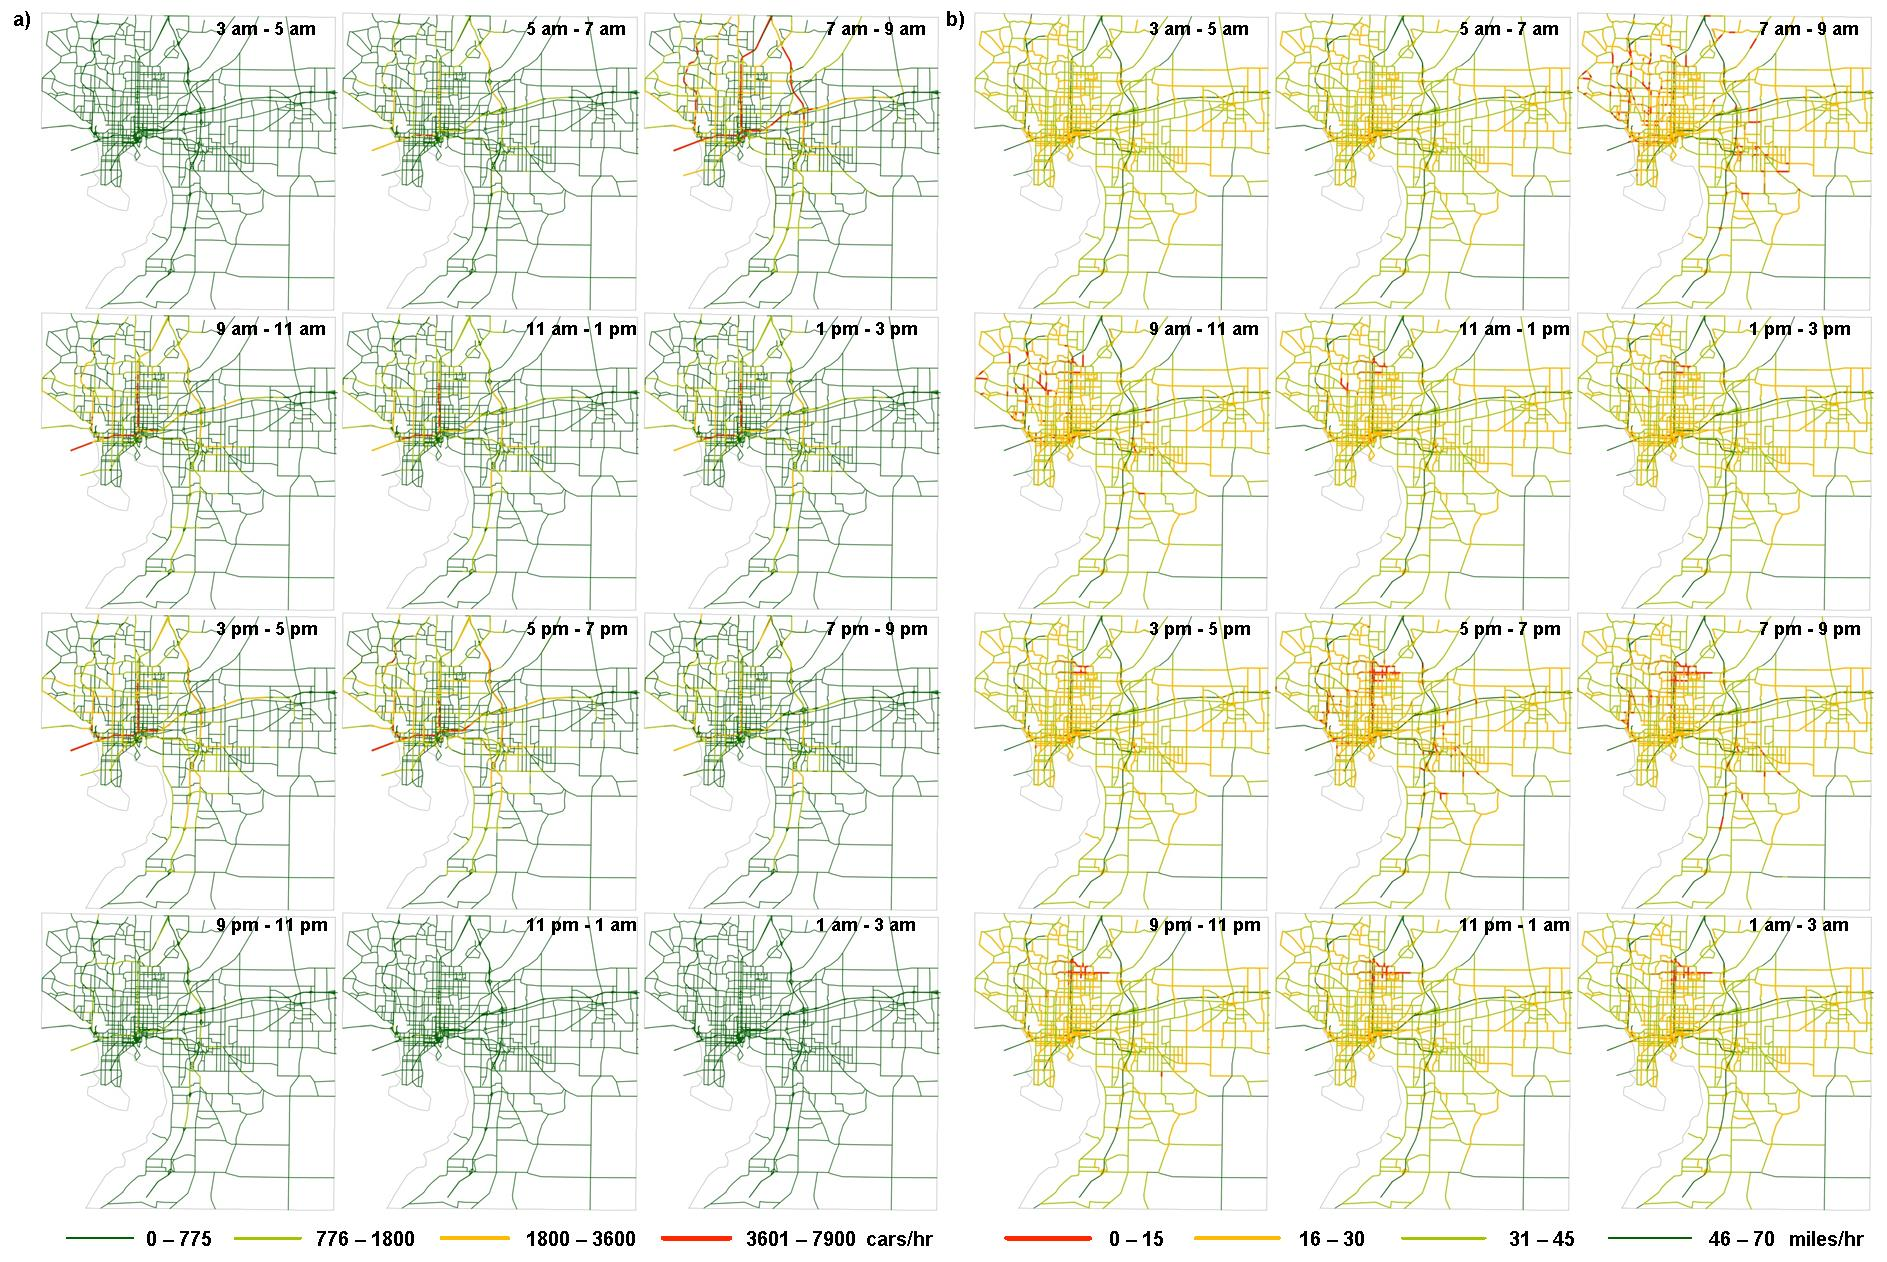
\includegraphics[width=1.5\textwidth, angle=90]{./scenarios/figures/tampa-fig3.jpg}}%
{}
 %------------

% ##################################################################################################################
\section{Future Work}
The next steps of this study include addition of inter-city, visitor, and freight travel to the model system. 
Utilizing the fine-resolution, link-level traffic volume and speed outputs from \gls{matsim}, EPA’s MOVES software is being used to estimate mobile source emissions. 
Mobile source emissions can be combined with other, point sources of emission as well as meteorological factors using a pollutant dispersion model to estimate diurnal cycles of hourly varying pollutant concentrations. 
The resulting pollutant concentrations (from the pollutant dispersion model) will be combined with the diurnal locations of individuals (obtained from \gls{abm} and \gls{matsim}) to estimate individual-level exposure to traffic-related pollutants such as nitrogen oxides. 
Such individual-level exposure measures will be utilized to estimate demographic group-level exposures for subsequent assessment of inequality in exposure to traffic-related air pollution as we have done previously using travel survey data \citep[][]{GurramEtAl_AQAH_2015}. 
The above described model system will be used to obtain estimates of population exposure for alternative scenarios of urban land-use design and transport policies.

% ##################################################################################################################
\section{Conclusion}
In this study, we simulated urban travel using activity-based travel demand modeling and \gls{dta}, to obtain network performance measures, including link-level traffic volumes and speeds, at a high spatial and temporal resolution for Hillsborough County in Florida. 
As expected, the simulated traffic volumes are higher and the travel speeds are lower during the morning and evening peak hours than other time periods in the day. 
Spatially, higher volumes and lower speeds are observed along the freeway corridors and suburban locations than other locations. 
Model performance (vis-à-vis observed traffic patterns) is better for inter-city roads compared to intra-city roads highlighting the need for better modeling of long distance passenger travel and freight movement. 
When the \gls{abm}-\gls{dta} framework built in this study is expanded to consider mobile source emissions and pollutant dispersion, the resulting transportation and air pollution modeling system will be useful for understanding interactions between urban transportation design, air pollution, and population exposure to pollution.

% ##################################################################################################################
